Il \textit{Data Collector} è un componente fondamentale dell'applicazione. Infatti, esso è adibito alla raccolta dei dati ottenuti grazie alle API selezionate nell'iterazione 0. In particolare, in questa iterazione si è stabilito di dedicarsi dell'implementazione della raccolta dei dati meteorologici tramite l'invocazione dell'API messa a disposizione del sito APRS.FI ( \url{https://aprs.fi/}) e descritta nel paragrafo \ref{par:APRSAPI}\todo{inserire terremoti e altro nel caso implementiamo}. 

Si è scelto di implementare questo componente come una applicazione scritta in Python, che verrà poi distribuita su un Raspberry Pi, in modo da garantire l'esecuzione continua. Per descriverne il funzionamento, si è costruito il diagramma di flusso rappresentato di seguito (\Fig\ref{fig:DCFlowChart}). Inizialmente, l'applicazione tenta la creazione di una connessione con il database. Se si verificano errori, il sistema attenderà 15 secondi prima di effettuare un nuovo tentativo di connessione. In questo modo, se si dovessero presentare problemi, come mancanza di connessione internet o irraggiungibilità del DB, il sistema effettuerà un nuovo tentativo di connessione. Una volta stabilita una connessione con il DB, vengono recuperati tutti i codici identificativi delle stazioni meteo (al massimo uno per ogni zona). Successivamente, viene avviato un thread per ogni zona, che si occuperà di recuperare i dati meteorologici dall'API, attraverso una chiamata HTTP di tipo GET. Una volta ricevuta la risposta in formato JSON, viene confrontata la data dell'acquisizione ricevuta con quella dell'ultima misurazione disponibile già inserita. Se essa coincide, il thread termina la sua esecuzione, altrimenti procede all'inserimento nel DB della nuova acquisizione. Questo controllo è stato inserito poiché le stazioni non hanno frequenze di aggiornamento uguali e costanti. In questo modo, si evita di memorizzare più volte la medesima acquisizione. Dopo aver salvato le informazioni nel database, viene attesa la terminazione di tutti i thread avviati e viene chiusa la connessione con il DB. Il programma attende 9 minuti prima di ricominciare il ciclo. 

\begin{figure}[h!]
	\centering
	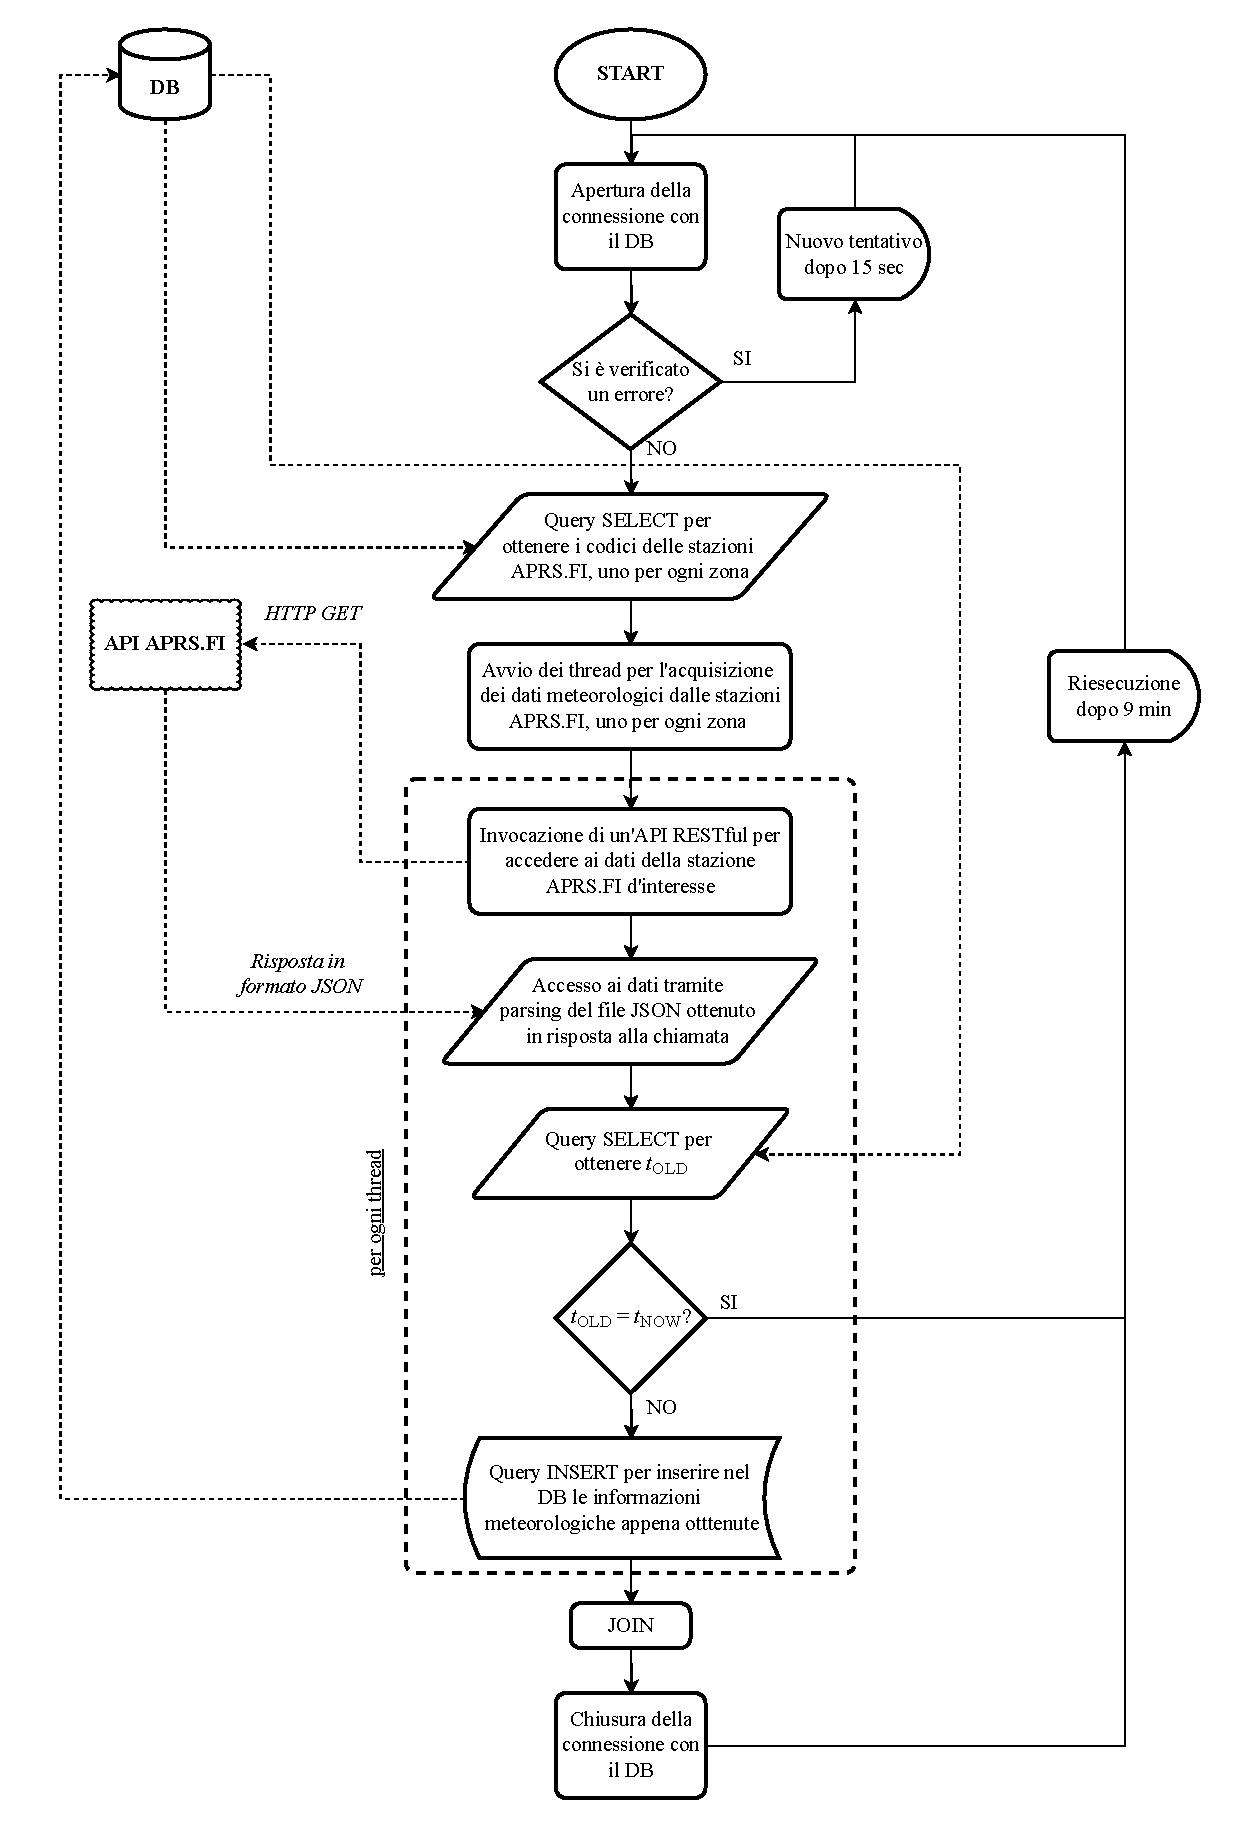
\includegraphics[width=1\linewidth]{./Iterazione 3/OtherFiles/FC - data collector}
	\caption{Diagramma di flusso di esecuzione del componente Data Collector.}
	\label{fig:DCFlowChart}
\end{figure}